\begin{figure*}[t]
    \centering
    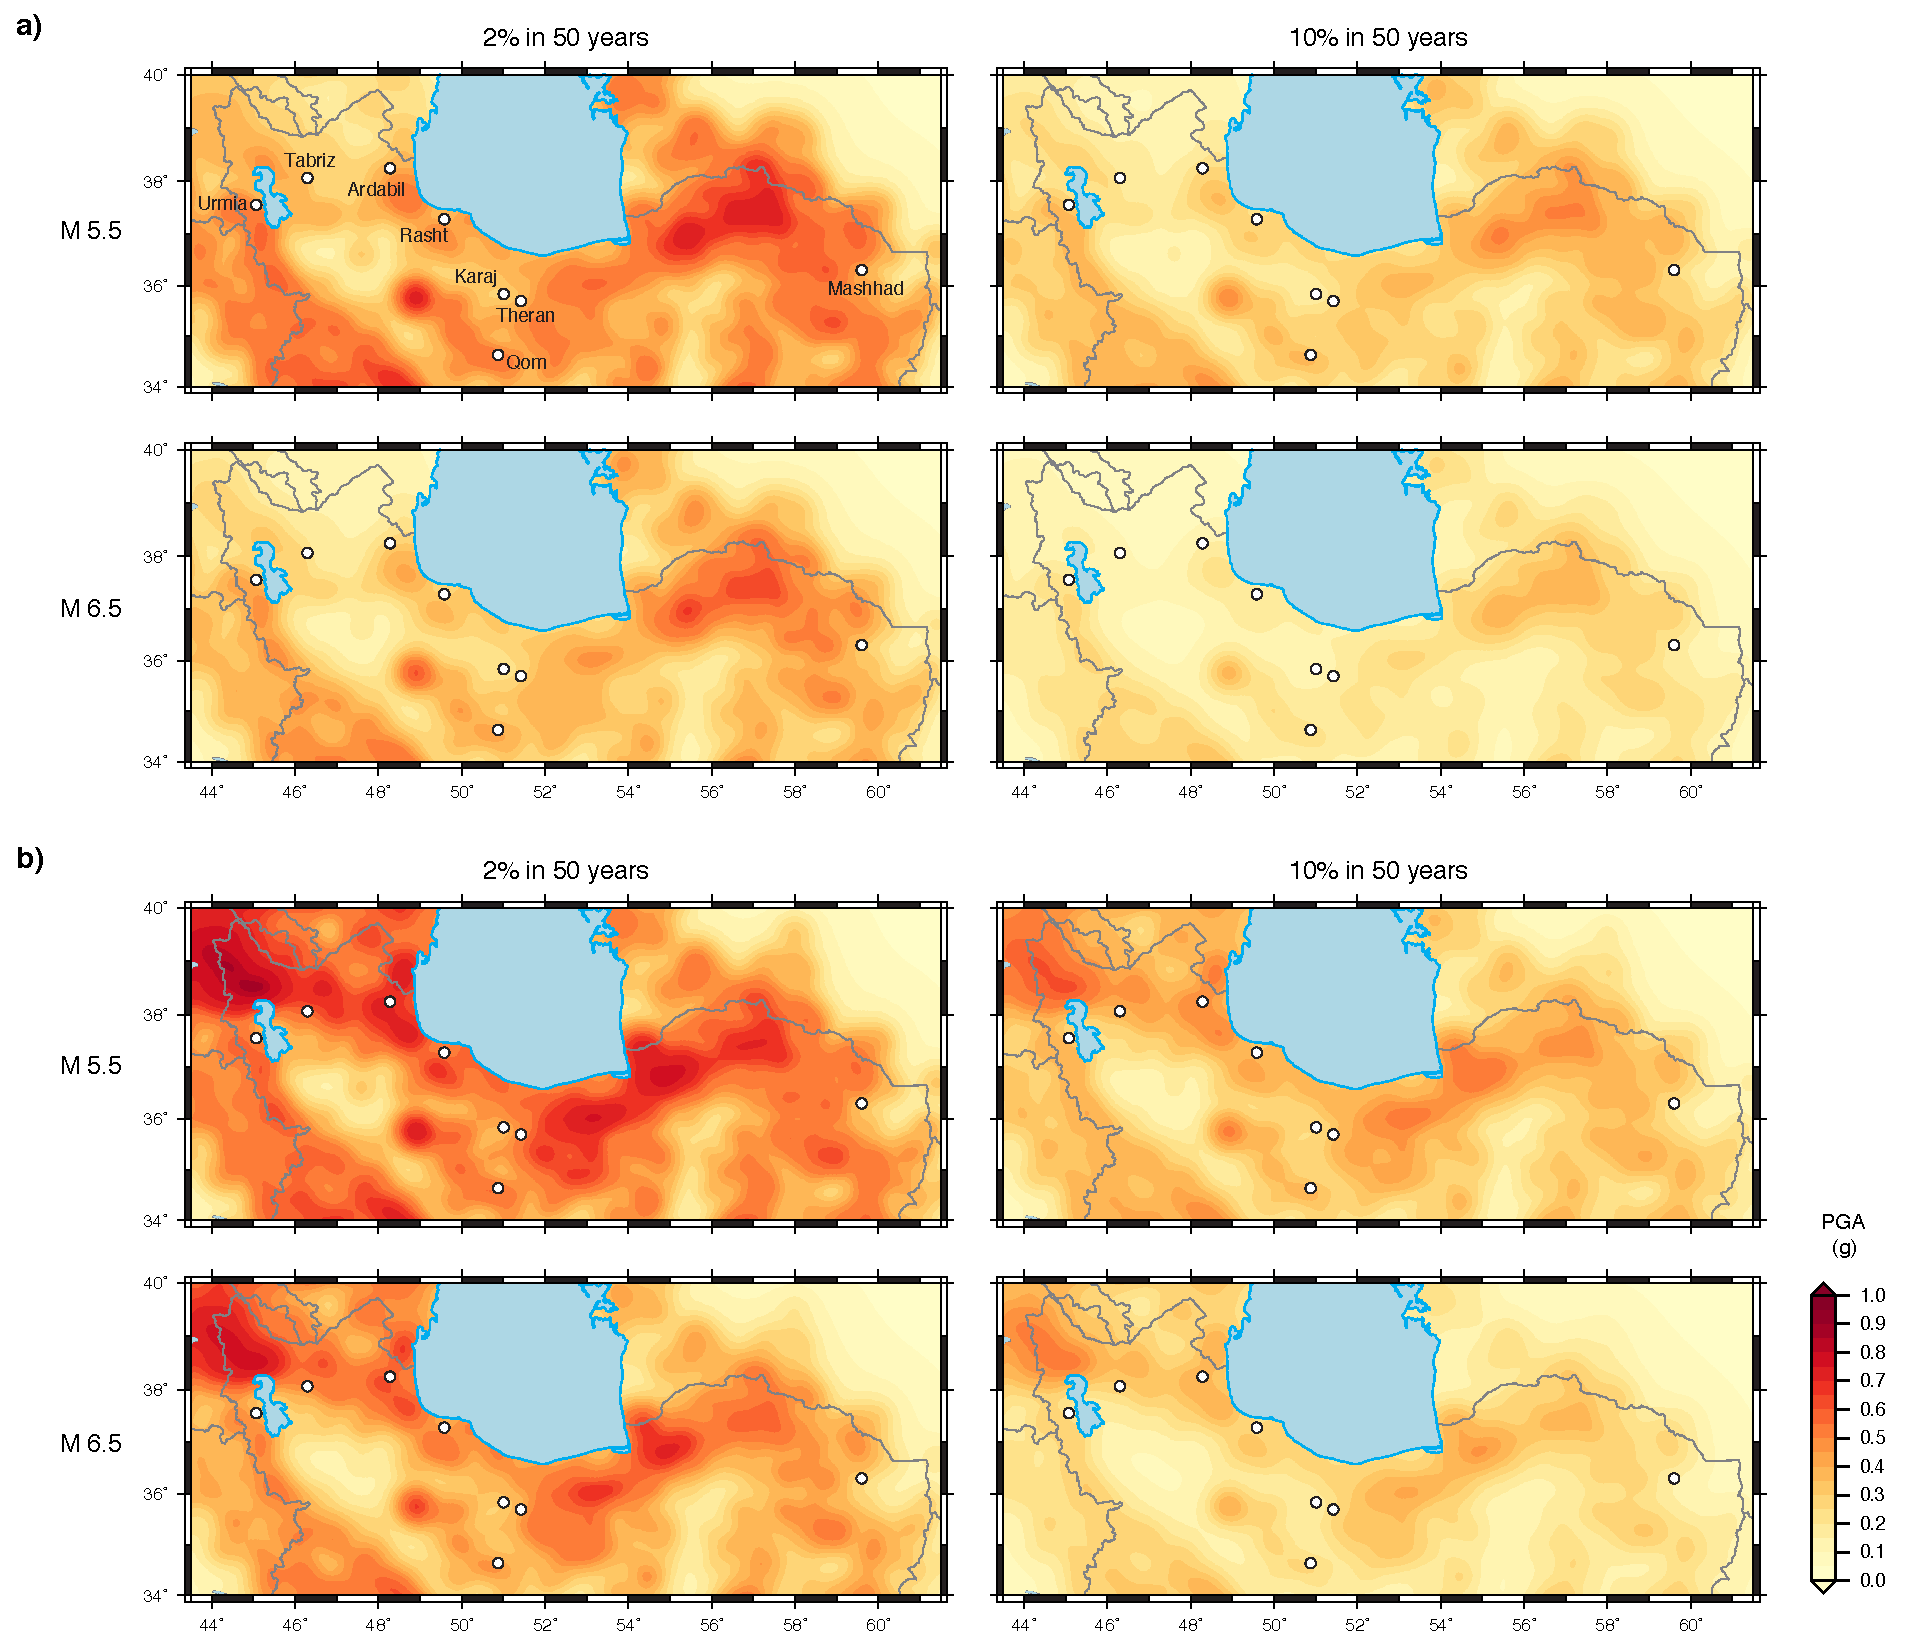
\includegraphics[width=\textwidth]{figures/pdf/figure-08} 
    \caption{Variation of horizontal peak ground acceleration (PGA) with distance. KG2004: \citet{Kalkan2004}, BA2008: \citet{Boore2008}, AB2010: \citet{Akkar2010}, SO2012: \citet{Soghrat2012}. The dashed line are $\pm$uncertainty of KG2004.}
    \label{fig:att}
\end{figure*}

\begin{figure*}[t]
    \centering
    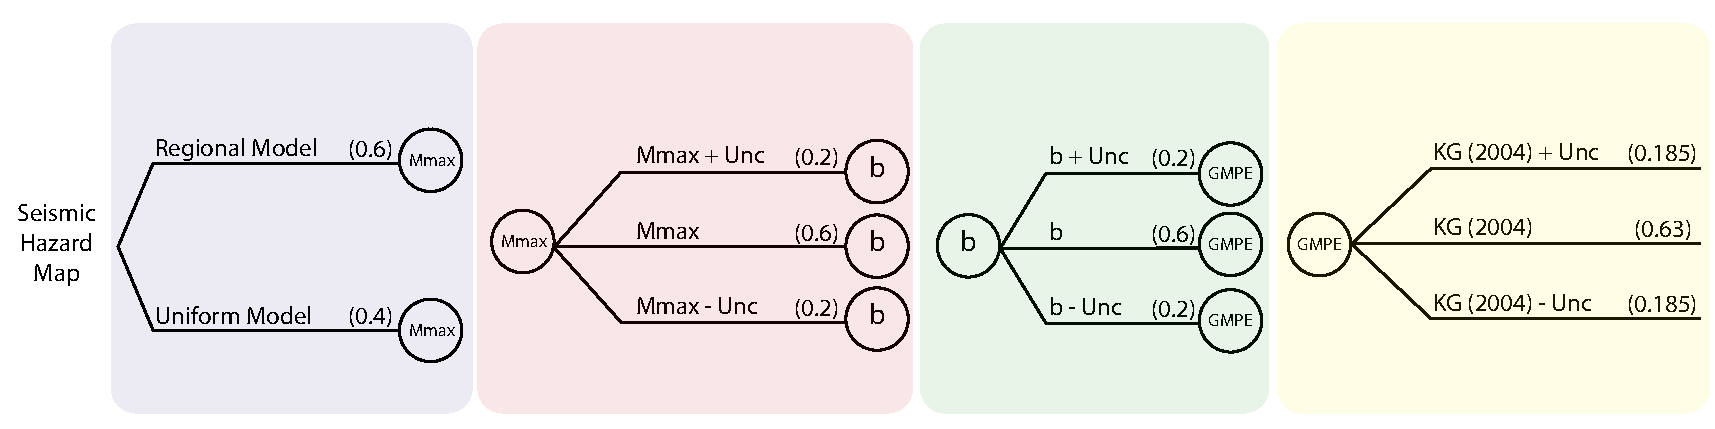
\includegraphics[width=\textwidth]{figures/pdf/figure-09}
    \caption{Logic tree for seismic hazard component in the North Iran.}
    \label{fig:logic}
\end{figure*}



\section{Attenuation Relationship}

The last piece in our hazard analysis process is the choice of an adequate attenuation relationship, or ground motion prediction equation (GMPE). This is a highly influential factor because it controls \myrevision{the intensity level at a particular site given earthquake locations and magnitude from the source model.}

Recently, \citet{Zafarani2014} investigated the predictive capabilities of a set of nine local, regional, and next generation attenuation (NGA) GMPEs to determine their applicability for northern Iran. They evaluated GMPE predictions against data from 32 earthquakes of magnitudes $M_w$ ranging between 4.7 and 7.4. This included comparisons of PGA and response spectral accelerations (SA) computed from time-series recorded on 163 stations located at epicentral distances of up to 200 km. The evaluation was done using the likelihood (LH) and log-likelihood (LLH) methods of \citet{Scherbaum_2004_BSSA, Scherbaum_2009_BSSA}. The combined evaluation for PGA, and SA for seven periods (T) between 0.1 and 2.0 s, yielded that the best overall predictions were those of the GMPEs introduced by \citet{Ghasemi_2009_JS}, \citet{Abrahamson_2008_ES}, and \citet{Chiou2008}. For the specific case of PGA ($T=0$ s), however, the best results were those obtained with the GMPEs introduced by \citet{Kalkan2004}, \citet{Chiou2008}, and \citet{Boore2008}. \myrevision{\citet{Soghrat2012} and \citet{Akkar2010} are other attenuation relationships which provide higher scores.}

Since our hazard analysis here focuses on PGA values only, we concentrated our attention in the last set of GMPEs. In comparisons not shown here for brevity, we found that these GMPEs yielded mean predictions that were very close to each other.\myrevision{ Fig.~\ref{fig:att} illustrates the variation of horizontal components pga (in g) with distance for four different magnitude. In practice, epistemic uncertainty is being considered by using different GMPEs through logic tree approach. As \citet{Atkinson2014} suggested, in most cases multiple-GMPEs approach is not necessarily acknowledge the epistemic uncertainty. This fact is also obvious from the Fig.~\ref{fig:att} where the alternative approach which is using \citet{Kalkan2004} as a backbone GMPE as well as uncertainties covers a broader range in compare with using the combination of GMPEs.} Furthermore, based on the LLH coefficients reported by \citet{Zafarani2014}, and using the \myrevision{approach} of \citet{Scherbaum_2009_BSSA}, we found that a logic-tree analysis \myrevision{leads} to weights of 0.3376, 0.3354, and 0.3270 for \citet{Kalkan2004}, \citet{Chiou2008}, and \citet{Boore2008}, respectively. These results meant that neither of them had a substantial advantage over the others. \myrevision{Fig.~\ref{fig:logic} represents the total logic tree approach in order to consider the uncertainty in tectonic seismic region, $M_{max}$, $b-value$, and estimated PGA. The weights are chosen based on previous studies \citep[e.g.,][]{Petersen2015}. We considered the uncertainty in tectonic seismic region through adding the uniform model with lower weight than the most recent accepted classification.}

Based on this, we selected the GMPE proposed by \citet{Kalkan2004} for our analysis. This equation is of the form
%
\begin{align}
	\ln \left( Y \right) =
		& \hspace{1ex} b_1 + b_2(M_w - 6) + b_3 \left( M_w - 6 \right)^{2} \nonumber \\
		& + b_5 \ln \left( r \right) + b_V \ln \left( V_S / V_A \right)
	\, ,
\end{align}
%
where $Y$ is a ground motion parameter (here representing PGA), $V_A$ is a reference velocity in m/s, \myrevision{and} $V_S$ is the shear wave velocity of the site of interest. In this equation, the distance $r$ is given by
%
\begin{equation}
	r= \sqrt{ r^2_{\mathit{cl}} + h^2 }
	\, ,
\end{equation}
%
where $r_{\mathit{cl}}$ is the horizontal distance to the site of interest and $h$ is a reference fictitious depth, both given in km. According to \citet{Kalkan2004}, in the case of $Y$ representing PGA, the coefficients $b_1$, $b_2$, $b_3$, $b_5$ and $b_V$ are
%
\begin{equation}
\begin{array}{lcrlcr}
	b_1 &=&  0.393   \,,&\hspace{2em}   b_2 &=& 0.576\,,   \\
	b_3 &=& -0.107   \,,&\hspace{2em}   b_5 &=& -0.899\,,  \\
	b_V &=& -0.200   \,;
	\nonumber
\end{array}
\end{equation}
%
and $V_A$, $V_S$ and $h$ are
%
\begin{equation}
\begin{array}{lcrl}
	V_A &=& 1,112 & \mathrm{m/s}	\\
	V_S &=&   700 & \mathrm{m/s}	\\
	h   &=&  6.91 & \mathrm{km}\,,
	\nonumber
\end{array}
\end{equation}
%
respectively. The standard deviation of the residuals $(\sigma_{\ln y})$ expressing the random variability of the ground motions is 0.612. The value of $V_S$ is assumed to represent average surface rock sites.

We should note here that even though \citet{Kalkan2004} derived the above attenuation relationship for distances $r$ up to 250 km, \citet{Zafarani2014} only used data up to 200 km in their evaluation of the various GMPEs available. Therefore, to be consistent with the latter, we set the models in the hazard analysis to compute ground motions (i.e., PGAs) at distances no greater than 200 km.
